% This is a template for our talks
\documentclass[12pt,english,dvipsnames]{beamer}
%\usetheme{Frankfurt}
\usepackage{sosy-beamer}
% \usepackage[scaled=0.8]{beramono}
\usepackage{amssymb,amsmath,mathtools}
\usepackage{tabto}
\usepackage{tikz}
\usetikzlibrary{cd}

\newcommand{\red}[1]{{\color{red}#1}}
\newcommand{\blue}[1]{{\color{blue}#1}}
\newcommand{\green}[1]{{\color{cpacheckergreen}#1}}
\newcommand{\Yes}{\green{\cmark}}
\newcommand{\No}{\red{\xmark}}

\newcommand{\code}[1]{\text{\upshape\ttfamily#1}}
\newcommand{\graycode}[1]{\code{\color{darkgray}#1}}
\newcommand{\low}{\code{low}}
\newcommand{\high}{\code{high}}
\newcommand{\id}{\mathit{id}}
\newcommand{\fp}{\mathit{fp}}
\newcommand{\blob}{\mathit{pk}}
\newcommand{\fingerprint}{\code{fingerprint}}
\newcommand{\haslabel}{\mathbin{\dblcolon}}
\newcommand{\Key}[2]{\code{Key}(#1,\,#2)}

\newcommand{\hoare}[3]{\{ #1 \}~~#2~~\{ #3 \}}
\newcommand{\loweq}{\equiv_\low}

\newcommand{\True}{\texttt{true}}
\newcommand{\False}{\texttt{false}}


\author{Gidon Ernst \inst{1}\and Toby Murray\inst{2} \and Mukesh Tiwari\inst{2}}
\title{Formal Specification and Information Flow}
\subtitle{VerifyThis long-term challenge 2020}

\institute{\inst{1}LMU Munich \and \inst{2} University of Melbourne, Australia}
\date{}


\begin{document}

\begin{frame}
    \centering
    {\Large \inserttitle}
    \bigskip

    {       \insertsubtitle}

    \bigskip

    \begin{minipage}[b]{2.5cm}
      \centering
    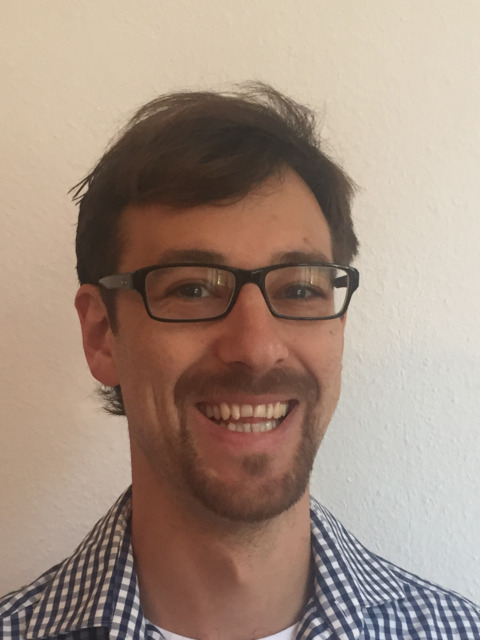
\includegraphics[height=2.5cm]{images/gernst.jpg} \\
    Gidon Ernst
    \end{minipage}
    \quad
    \begin{minipage}[b]{2.5cm}
      \centering
    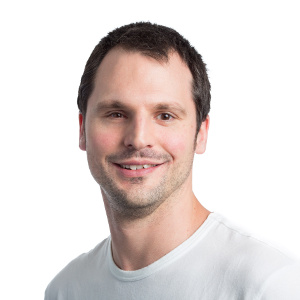
\includegraphics[height=2.5cm]{images/TobyMurray.jpg} \\
    Toby Murray
    \end{minipage}
    \quad
    \begin{minipage}[b]{2.5cm}
      \centering
    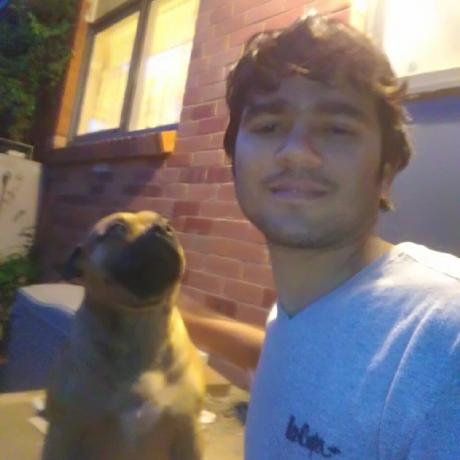
\includegraphics[height=2.5cm]{images/MukeshTiwari.jpg} \\
    Mukesh Tiwari
    \end{minipage}

    \bigskip

    \mailto{gidon.ernst@lmu.de} \quad \mailto{toby.murray@unimelb.edu.au}  
    \quad \mailto{mukesh.tiwari@unimelb.edu.au}\\
    \url{github.com/mukeshtiwari/VerifythisSpecification}
\end{frame}

\begin{frame}
\frametitle{Big Ideas}
\begin{itemize}
	\item What are we trying to achieve here
	\item Why did we formally specify in Coq/Isabelle
	\item Future plans

\end{itemize}

\end{frame}




\end{document}
